%% fancy header & foot
\pagestyle{fancy}
\lhead{[ELEC-H-2001] Électricité\\ Séance \no 11 : Séance récapitulative - Théorie des champs \ifthenelse{\boolean{corrige}}{~-- corrigé}{}}
\rhead{v1.0.0\\ page \thepage}
\cfoot{}
%%

\pdfinfo{
/Author (Renaud Theunissen et Youssef Agram, ULB -- BEAMS-EE)
/Title (Séance 11 ELEC-H-2001, Séance récapitulative - Théorie des champs)
/ModDate (D:\pdfdate)
}

\hypersetup{
pdftitle={Séance 11 [ELEC-H-2001] Électricité : Séance 10 ELEC-H-2001, Séance récapitulative - Théorie des champs},
pdfauthor={Renaud Theunissen et Youssef Agram, ©2020 ULB - BEAMS-EE},}

\setlength{\parskip}{0.5cm plus4mm minus3mm} %espacement entre §
\setlength{\parindent}{0pt}


\begin{document}
\long\def\nothx/*#1*/{}
\tptitle{}{Séance 11~: Séance récapitulative - Théorie des champs}
\section{But de la séance}
L'objectif de cette séance est de vous proposer des questions de résolution pratique typiques d'examen pour la partie théorie des champs.
Cette séance sert de synthèse aux séances d'exercices consacrées aux champs.

\section{Pré-requis}
Avant la séance, vous aurez relu les chapitres et sections suivants:
\begin{itemize}
	\item Chapitre 2 - Électrostatique dans le vide 
		\begin{itemize}
		\item Section 2.2 - Champ électrique
		\item Section 2.3 - Potentiel électrique
		\item Section 2.6 - Conditions aux limites de part et d'autres d'une surface chargée
		\item Section 2.7 - Condensateur et coefficient de capacité
		\item Section 2.9 - Dipôle électrique
		\end{itemize}
	\item Chapitre 3 - Milieux diélectriques
		\begin{itemize}
		\item Section 3.2 - Matériaux diélectriques et polarisation
		\item Section 3.3 - Champs de déplacement $\Vec{D}$ et relation constitutive
		\item Section 3.4 - Diélectriques linéaires
		\item Section 3.6 - Conditions aux limites
		\item Section 3.8 - Condensateur plan et diélectrique 
		\item Section 3.9 - Expression générale du coefficient de capacité
		\end{itemize}
	\item Chapitre 4 - Milieux conducteurs (effet résistif)
		\begin{itemize}
		\item Section 4.1 - Tension et courant
		\item Section 4.2 - Relation constitutive : loi d'Ohm locale
		\item Section 4.3 - Coefficient de résistance
		\item Section 4.5 - Conditions aux limites
		\item Section 4.7 - Puissance dissipée : effet Joule
		\item Section 4.8 - Exemples de calcul de résistance
		\end{itemize}
	\item Chapitre 5 - Magnétostatique dans le vide
	    \begin{itemize}
	        \item Section 5.2 - Champ magnétique 
	        \item Section 5.5 - Formule de Biot et Savart
	        \item Section 5.6 - Conditions aux limites de part et d'autre d'une surface parcourue par un courant
	        \item Section 5.9 - Coefficient d'inductance
	        \item Section 5.12 - Forces et couples sur des courants
	    \end{itemize}
	\item Chapitre 6 - Milieux magnétiques
	    \begin{itemize}
	        \item Section 6.2 - Matériaux magnétiques et magnétisation
	        \item Section 6.3 - Champ magnétisant $\Vec{H}$ et relation constitutive
	        \item Section 6.4 - Milieux magnétiques linéaires
	        \item Section 6.5 - Origine physique de la magnétisation (interprétation des courants de magnétisation)
	        \item Section 6.6 - Conditions aux limites
	        \item Section 6.8 - Ferromagnétisme
	    \end{itemize}
	\item Chapitre 8 - Circuits magnétiques : une autre sorte de circuits
	    \begin{itemize}
	        \item Section 8.1 - Équivalence entre milieux conducteurs et milieux magnétiques 
	        \item Section 8.2 - Réluctance
	        \item Section 8.3 - Transposition de la théorie des circuits
	        \item Section 8.4 - Calcul de flux et d'inductance via la réluctance (exemples)
	        \item Section 8.5 - Transformateurs
	    \end{itemize}
\end{itemize}

\vspace{5pt}

\newpage

\section{Théorie des champs - Exercices d'examens}
\subsection{Examen Janvier 2019 (Q1)}

Une particule chargée, de charge Q et de masse m, est lancée avec une vitesse v entre 2 plaques planes connectées à une source de tension continue $V_0$. La particule est déviée et percute un écran de détection située à une distance L du bord des 2 plaques chargées.
Les plaques sont carrées de côtés de longueur a et sont espacées d’une distance d. \\
La situation est illustrée ci-dessous avec les données numériques.
\begin{figure}[h!]
    \centering
    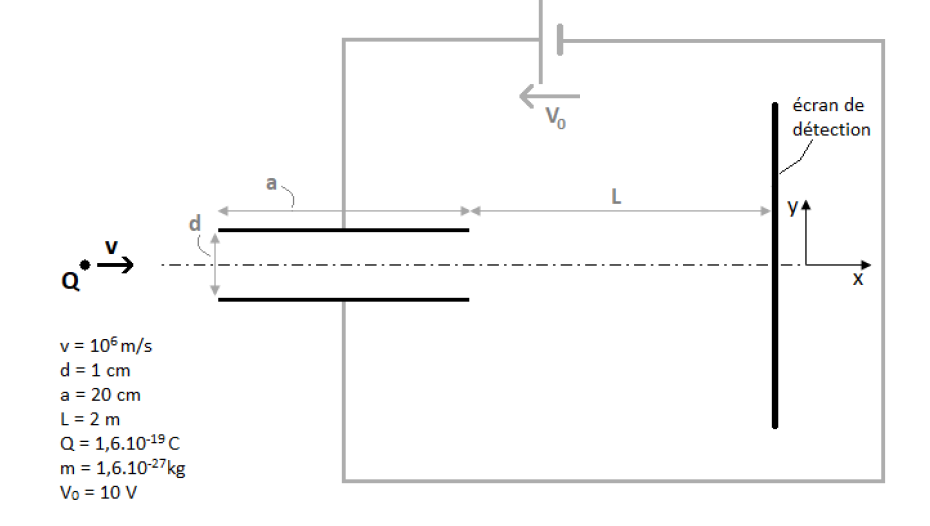
\includegraphics[width = 17cm]{TpQEx_Champs/Q1_TheoChampsJanv2019.PNG}
    %\caption{}
    \label{fig:Q1_TheoChampsJanv2019}
\end{figure}

\Question{
\newline
Calculer la position de détection y sur l’écran de détection en fonction des paramètres du système. Donner également sa valeur numérique. Utiliser le système d’axe donné sur le schéma (y positif vers le haut, avec l’origine au centre de l’écran de détection). \\\textbf{Négliger les effets de bords.}
}
{%C
}
\newpage
\subsection{Examen Janvier 2018 (Q1)}
Soit une spire circulaire de rayon R parcourue par un courant I. Soit une autre spire carrée ouverte de côté a. Les 2 spires sont éloignées d’une distance D l’une de l’autre et sont parallèles entre elles. \\
La situation est illustrée ci-dessous.
\begin{figure}[h!]
    \centering
    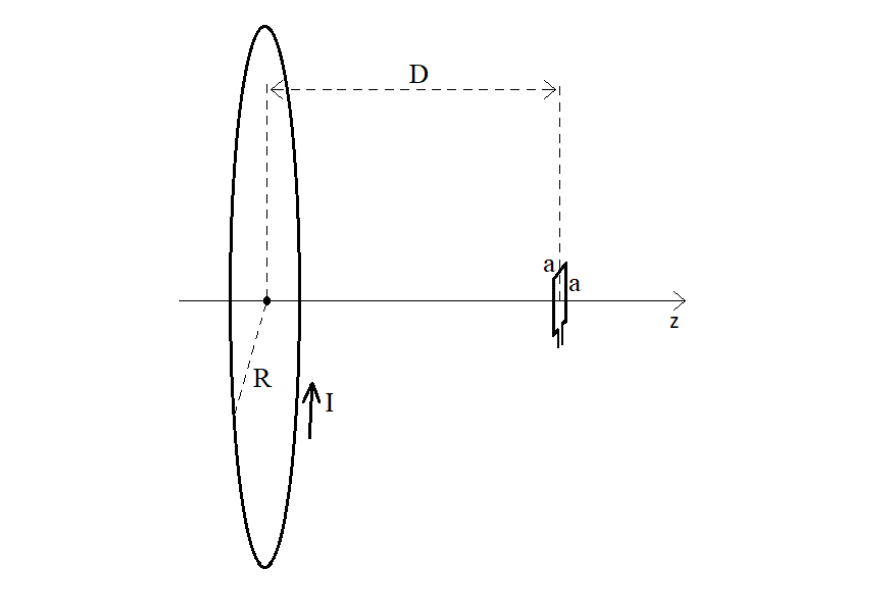
\includegraphics[width = 15cm]{TpQEx_Champs/Q1_TheoChampsJanv2018.PNG}
    %\caption{}
    \label{fig:Q1_TheoChampsJanv2018}
\end{figure}

\begin{enumerate}
    \item Calculer le champ magnétique ~B le long de l’axe z.
    \item Supposant la valeur de B constante sur la petite spire carrée (égale à la valeur au centre de la spire), calculer le flux capté par cette spire carrée ainsi que le coefficient d’inductance mutuelle entre les 2 spires.
    \item Calculer la tension induite e(t) induite sur la spire carrée si celle-ci se déplace à une vitesse constante v en direction de la spire circulaire. Supposer toujours que la valeur de B est constante sur la spire.
\end{enumerate}

\newpage
\subsection{Examen Janvier 2016 (Q2)}
Soit une sphère de rayon a. Cette sphère est constituée de 2 demi-sphères uniformément chargées d’une charge +Q et -Q. La situation est représentée ci-dessous. Le milieu dans lequel se trouve la sphère est le vide.\\
La situation est illustrée ci-dessous.
\begin{figure}[h!]
    \centering
    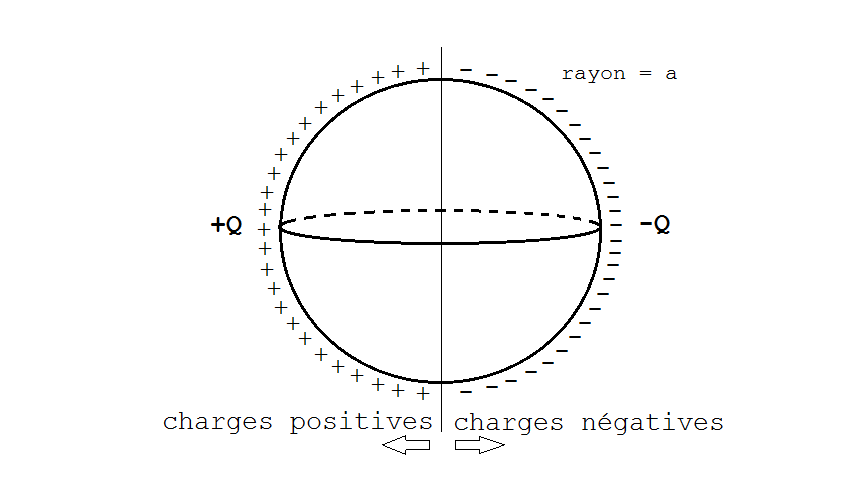
\includegraphics[width = 14cm]{TpQEx_Champs/Q2_TheoChampsJuin2016.PNG}
    %\caption{}
    \label{fig:Q2_TheoChampsJuin2016}
\end{figure}
Pour rappel :
\begin{figure}[h!]
    \centering
    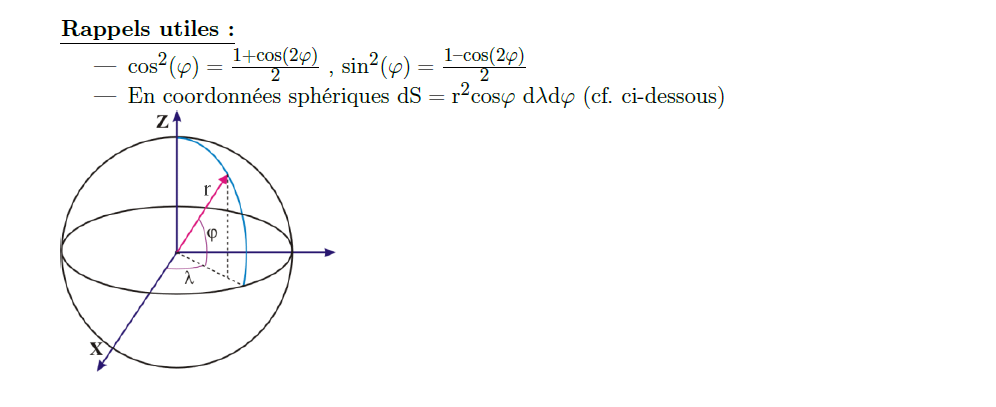
\includegraphics[width = 18cm]{TpQEx_Champs/Q2_Hint_TheoChampsJuin2016.PNG}
    %\caption{}
    \label{fig:Q2_Hint_TheoChampsJuin2016}
\end{figure}

\begin{enumerate}
    \item Le problème présente-t-il une symétrie sphérique ? Justifier.
    \item Est-ce que la sphère est parfaitement conductrice ? Justifier.
    \item Calculer la densité surfacique de charge $\sigma$ de chaque côté de la sphère.
    \item Que vaut le potentiel électrique V au centre de la sphère ? Justifier.
    \item Que vaut le champ électrique ~E au centre de la sphère ? Donner son amplitude, sa direction et son sens.
\end{enumerate}

\newpage
\subsection{Examen Septembre 2018 (Q2)}
Soient 2 fils chargés uniformément, l’un d’une densité linéique de charge $\rho$ et l’autre d’une densité $-\rho$ ($\rho > 0$). Les fils sont séparés par une distance d (entre leur centres), leur rayon est égal à a et ils sont de longueur infinie. Le système est plongé dans un milieu assimilable au vide. 
Le matériau des fils est un métal parfait.
\begin{figure}[h!]
    \centering
    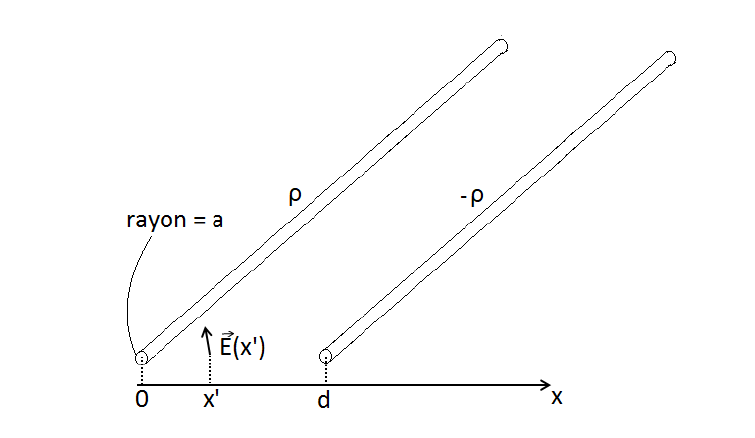
\includegraphics[width = 15cm]{TpQEx_Champs/Q2_TheoChampsSept2018.PNG}
    %\caption{}
    \label{fig:Q2_TheoChampsSept2018}
\end{figure}

\begin{enumerate}
    \item Calculer le champ électrique E existant entre les 2 conducteurs en fonction de $\rho$, d, a et x’. Supposer que $d \gg a$.
    \item Représenter qualitativement 3 lignes de champs électriques différentes sur le dessin ci-dessous. Représenter également la répartition des charges dans les 2 fils (via des "+" et des "-"). Les fils sont représentés par une vue en coupe, ils sont donc perpendiculaires à cette feuille.\\
    
    Que vaut le champ électrique à l’intérieur des fils ? 
    \begin{figure}[h!]
        \centering
        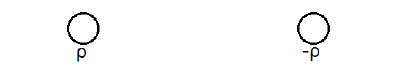
\includegraphics[width = 10cm]{TpQEx_Champs/Q2_Hint_TheoChampsSept2018.PNG}
        %\caption{}
        \label{fig:Q2_Hint_TheoChampsSept2018}
    \end{figure}
    \item Calculer la capacité par unité de longueur constituée par les 2 fils conducteurs.
\end{enumerate}

\newpage

\subsection{Examen Janvier 2020 (Q4)}

On considère le circuit magnétique suivant, constitué d’un matériau magnétique linéaire de perméabilité $µ_r$. 
\begin{figure}[h!]
    \centering
    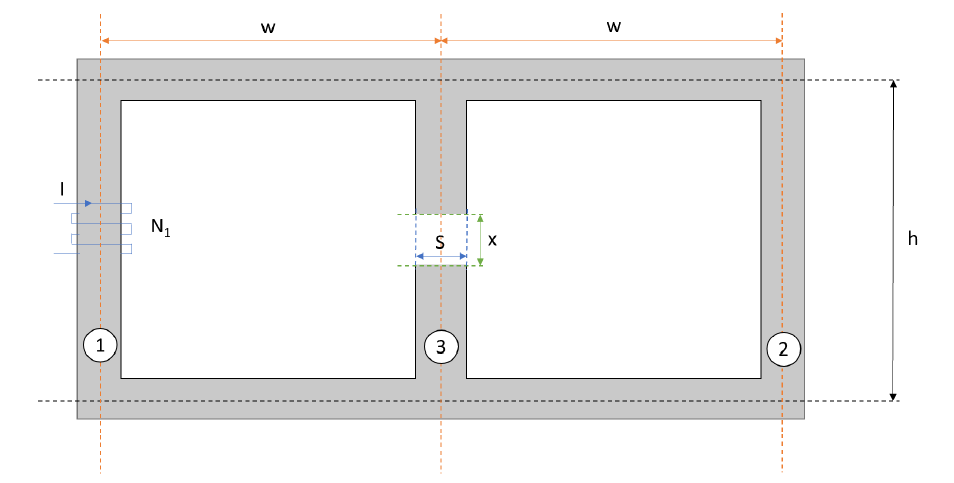
\includegraphics[width = 14cm]{TpQEx_Champs/Q4_TheoChampsJanv2020.PNG}
    %\caption{}
    \label{fig:Q4_TheoChampsJanv2020}
\end{figure}
Avec les hypothèses et caractéristiques suivantes :
\begin{figure}[h!]
    \centering
    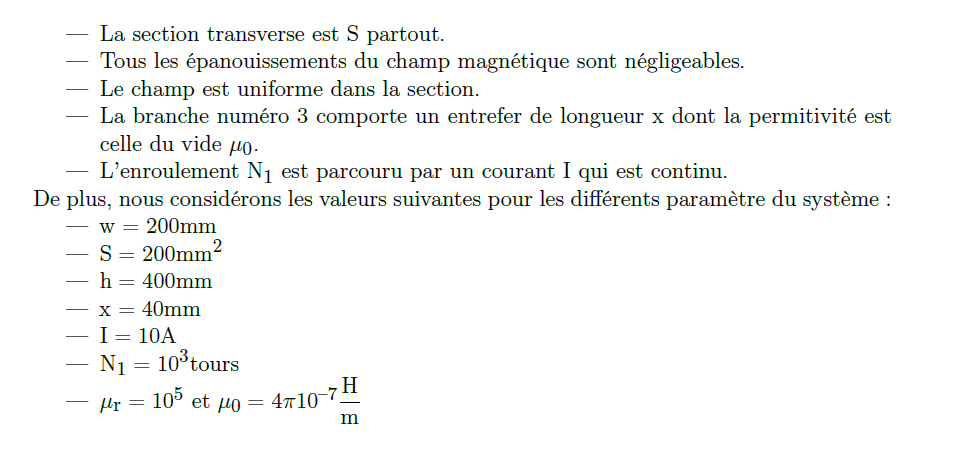
\includegraphics[width = 13cm]{TpQEx_Champs/Q4_Caracts_TheoChampsJanv2020.PNG}
    %\caption{}
    \label{fig:Q4_Caracts_TheoChampsJanv2020}
\end{figure}

\begin{enumerate}
    \item Calculez les réluctances des trois branches du circuit magnétique.
    \item Représentez le circuit électrique équivalent et déterminez le flux dans chaque branche du circuit magnétique.
\end{enumerate}

\newpage
\subsection{Examen Janvier 2017 (Q2)}

Soit le circuit à réluctances ci-dessous :
\begin{figure}[h!]
    \centering
    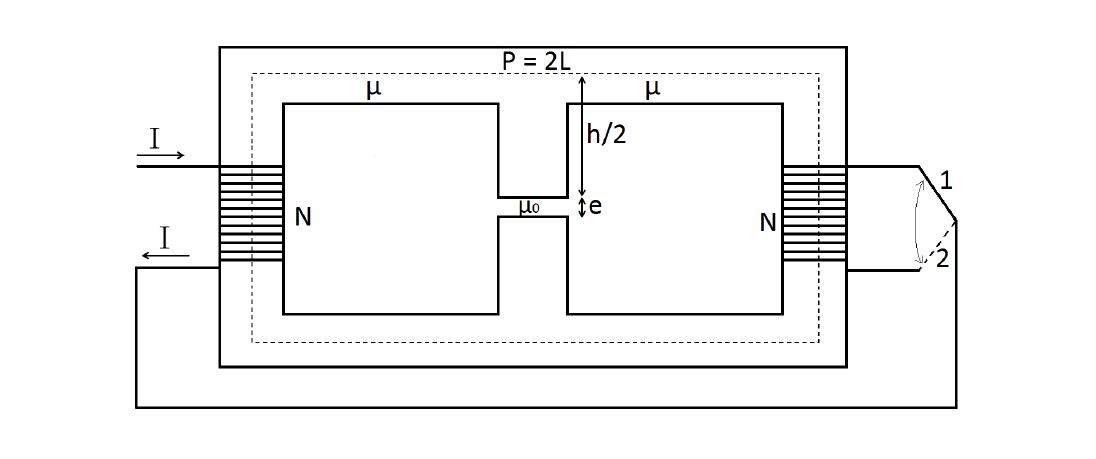
\includegraphics[width = 14cm]{TpQEx_Champs/Q2_TheoChampsJanv2017.PNG}
    %\caption{}
    \label{fig:Q2_TheoChampsJanv2017}
\end{figure}
Les données du système sont les suivantes :
\begin{figure}[h!]
    \centering
    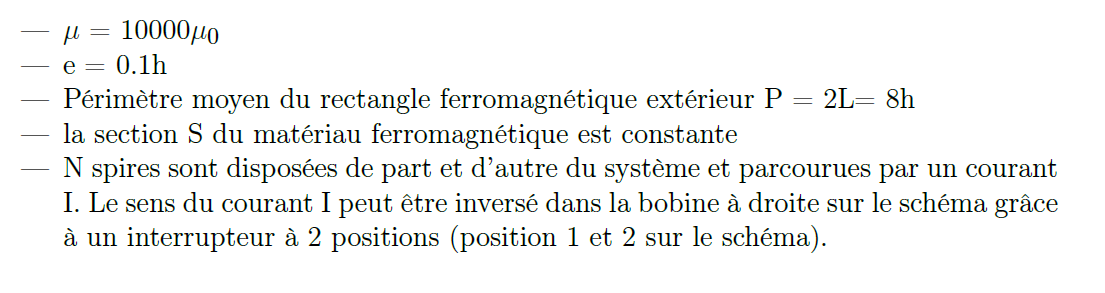
\includegraphics[width = 13cm]{TpQEx_Champs/Q2_Hint_TheoChampsJanv2017.PNG}
    %\caption{}
    \label{fig:Q2_Hint_TheoChampsJanv2017}
\end{figure}

\begin{enumerate}
    \item Calculer la réluctance du demi-périmètre de longueur L. Calculer également les 2 réluctances de la branche centrale (dans le matériau et dans
    l’air). Quelle réluctance est la plus grande ? Calculer le rapport entre la plus grande réluctance et les 2 autres.
    \item Pour les 2 positions de l’interrupteur, représenter le circuit électrique équivalent à ce circuit magnétique. Attention à bien définir tous
    les éléments et grandeurs du circuit ainsi que la position de l’interrupteur correspondant à chaque circuit.
    \item Pour les 2 positions de l’interrupteur, calculer le flux circulant dans le périmètre P du matériau ferromagnétique. Vous pouvez faire des hypothèses simplificatrices pour le calcul.
\end{enumerate}
\end{document}